% $Header: svn+ssh://andre@crapman/home/junda/repos/andre/school/trunk/m/Chapter/algebra.ii/ch04.matrices/matrices.main.tex 273 2021-10-02 20:40:50Z andre $

% touch ch01.basics/ch01.basics.tex
% svn add ch01.basics/ch01.basics.tex
% svn propset svn:keywords "Header" ch01.basics/ch01.basics.tex

\tikzsetfigurename{hydraulic.pneumatic.ch01}
% \tikzexternaldisable
% \tikzexternalenable

% \part{Kombi}
\section{Hydraulische und Pneumatische Bauteile}
\subsection{Literatur}
%= = = = = = = = = = = = = = = = = = = = = = = = = = = = = = = = = = = = = = =
%= = = = = = = = = = = = = = = = = = = = = = = = = = = = = = = = = = = = = = =
% \iffalse
\begin{frame}
  \frametitle{Literatur}
%  \framesubtitle{H\"oren}
  %%= = = = = = = = = = = = = = = = = = = = = = = = = = = = = = = = = = = = = =
  \textsc{Holger WALTER}\\
  {\Large\textbf{Hydraulik und Pneumatik}}\\
  Grundlagen und Übungen -
  Anwendungen und Simulation

  \vspace{3\baselineskip}
  \textsc{Beate BENDER \& Dietmar G\"OHLICH} (Hrsg.)\\
  {\Large\textbf{Dubbel Taschenbuch}}\\
  f\"ur den Maschinenbau 2:  Anwendungen
  {\small{}Kap. 18:
  Bauelemente hydrostatischer Getriebe v. 
  Dierk Feldmann und Stephan Bartelmei}

  %%= = = = = = = = = = = = = = = = = = = = = = = = = = = = = = = = = = = = = =

\end{frame}
%= = = = = = = = = = = = = = = = = = = = = = = = = = = = = = = = = = = = = = =


% \part{Kombi}
% \section{Hydraulische und Pneumatische Bauteile}
\subsection{Intro}
%= = = = = = = = = = = = = = = = = = = = = = = = = = = = = = = = = = = = = = =
%= = = = = = = = = = = = = = = = = = = = = = = = = = = = = = = = = = = = = = =
% \iffalse
\begin{frame}
  \frametitle{Intro}
%  \framesubtitle{H\"oren}
  %%= = = = = = = = = = = = = = = = = = = = = = = = = = = = = = = = = = = = = =
  \vspace{-0.3\baselineskip}
  Fluidtechnik: Hydraulik und Pneumatik überträgt Kraft und Leistung zum Antreiben, Steuern und 
  Bewegen. Bei 
  \begin{itemize}
    \item  linearen wie auch 
    \item  \adSTField{rotatorischen} Bewegungen, 
    \item  gleichmäßigen Hub oder \adSTField{Senkbewegungen}, 
    % \item  Beschleunigungsforderungen und
    \item  Positionierungen 
  \end{itemize}
  finden hydraulische und pneumatische \adSTField{Komponenten}
   in fast allen Bereichen der Industrie ihre Anwendung.
  
   \ifteacher%%
   \else%%
    %  \vspace*{-0.7\baselineskip}\hspace{\stretch{1}}\rotatebox[origin=lB]{180}{%%
     \vspace*{-1.0\baselineskip}\hspace{\stretch{1}}\rotatebox[origin=lB]{180}{%%
     \resizebox{0.9\linewidth}{!}{\parbox[t]{3.95\linewidth}{%%
    %  \tiny
   %   \vspace*{-0.7\baselineskip}\hspace*{0.95\linewidth-1cm}\makebox[0pt][l]{\rotatebox[origin=c]{180}{\resizebox{1cm}{!}{%
       rotatorischen, Senkbewegungen, Komponenten
     }}}
   \fi%%
  %%= = = = = = = = = = = = = = = = = = = = = = = = = = = = = = = = = = = = = =

\end{frame}
%= = = = = = = = = = = = = = = = = = = = = = = = = = = = = = = = = = = = = = =

% \part{Kombi}
% \section{Hydraulische und Pneumatische Bauteile}
% \subsection{Intro}
%= = = = = = = = = = = = = = = = = = = = = = = = = = = = = = = = = = = = = = =
%= = = = = = = = = = = = = = = = = = = = = = = = = = = = = = = = = = = = = = =
% \iffalse
\begin{frame}
  \frametitle{Intro}
%  \framesubtitle{H\"oren}
  %%= = = = = = = = = = = = = = = = = = = = = = = = = = = = = = = = = = = = = =
  
  Vorteile:
  \begin{itemize}
    \item hohe \adSTField{Leistungsdichte}: hohe Kräfte und Drehmomente bei 
      geringer Abmessungen (\adSTField{1:10} vs. E-Motor)
    \item stufenlose \adSTField{Geschwindigkeitsregelung}
    \item Hohe Last bei geringer \adSTField{Geschwindigkeit}
    \item geringe \adSTField{Trägheitsmassen} (1:50 vs. E-Motor)
    \item problemlose Verwendung in \adSTField{explosionsgefährdeten} Räumen
    \item einfacher und kostengünstiger Betrieb (\adSTField{Pneumatik} auch Anschaffung)
  \end{itemize}

\ifteacher%%
\else%%
 %  \vspace*{-0.7\baselineskip}\hspace{\stretch{1}}\rotatebox[origin=lB]{180}{%%
  \vspace*{-0.0\baselineskip}\hspace{\stretch{1}}\rotatebox[origin=lB]{180}{%%
  \resizebox{0.9\linewidth}{!}{\parbox[t]{3.95\linewidth}{%%
 %  \tiny
%   \vspace*{-0.7\baselineskip}\hspace*{0.95\linewidth-1cm}\makebox[0pt][l]{\rotatebox[origin=c]{180}{\resizebox{1cm}{!}{%
  Leistungsdichte, 1:10, Geschwindigkeitsregelung, Geschwindigkeit, Trägheitsmassen,  
  explosionsgefährdeten, Pneumatik
  }}}
\fi%%
  
  %%= = = = = = = = = = = = = = = = = = = = = = = = = = = = = = = = = = = = = =

\end{frame}
%= = = = = = = = = = = = = = = = = = = = = = = = = = = = = = = = = = = = = = =


% \part{Kombi}
% \section{Hydraulische und Pneumatische Bauteile}
% \subsection{Intro}
%= = = = = = = = = = = = = = = = = = = = = = = = = = = = = = = = = = = = = = =
%= = = = = = = = = = = = = = = = = = = = = = = = = = = = = = = = = = = = = = =
% \iffalse
\begin{frame}
  \frametitle{Intro}
%  \framesubtitle{H\"oren}
  %%= = = = = = = = = = = = = = = = = = = = = = = = = = = = = = = = = = = = = =
  
  Nachteile:
  \begin{itemize}
    \item hohe \adSTField{Pr\"azision} bei Bauteilen für Hydraulik notwendig, 
      daher hohe Anschaffungskosten
    \item geringe \adSTField{\"Ubertragungsentfernungen}
    \item geringe Effektivität, \adSTField{Schlupf} 
    \item hoher Aufwand für \adSTField{Umweltschutz}
  \end{itemize}
  
   \ifteacher%%
   \else%%
    %  \vspace*{-0.7\baselineskip}\hspace{\stretch{1}}\rotatebox[origin=lB]{180}{%%
     \vspace*{-1.0\baselineskip}\hspace{\stretch{1}}\rotatebox[origin=lB]{180}{%%
     \resizebox{0.9\linewidth}{!}{\parbox[t]{3.95\linewidth}{%%
    %  \tiny
   %   \vspace*{-0.7\baselineskip}\hspace*{0.95\linewidth-1cm}\makebox[0pt][l]{\rotatebox[origin=c]{180}{\resizebox{1cm}{!}{%
       Pr\"azision, \"Ubertragungsentfernungen, Schlupf, Umweltschutz
     }}}
   \fi%%
  
  %%= = = = = = = = = = = = = = = = = = = = = = = = = = = = = = = = = = = = = =

\end{frame}
%= = = = = = = = = = = = = = = = = = = = = = = = = = = = = = = = = = = = = = =

% \part{Kombi}
% \section{Hydraulische und Pneumatische Bauteile}
% \subsection{Intro}
%= = = = = = = = = = = = = = = = = = = = = = = = = = = = = = = = = = = = = = =
%= = = = = = = = = = = = = = = = = = = = = = = = = = = = = = = = = = = = = = =
% \iffalse
\begin{frame}
  \frametitle{Antriebe im Vergleich}
%  \framesubtitle{H\"oren}
  %%= = = = = = = = = = = = = = = = = = = = = = = = = = = = = = = = = = = = = =
  
  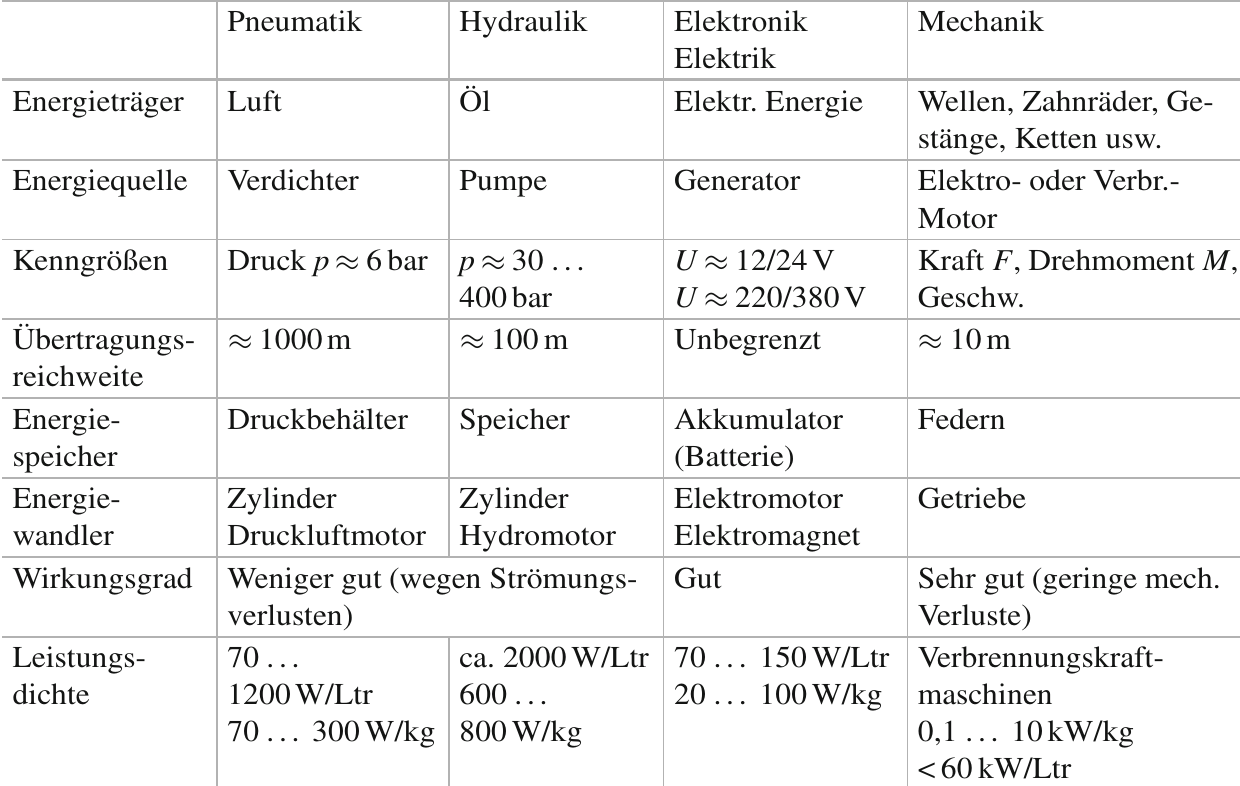
\includegraphics[width=\linewidth]{./ch01.basics/pics/compareDrives}  
  
  \vspace*{-1.0\baselineskip}{\tiny\color{red}Aus Sicherheitsgr\"unden wird bei der Pneumatik kein h\"oherer Druck 
  verwendet.}
  %%= = = = = = = = = = = = = = = = = = = = = = = = = = = = = = = = = = = = = =

\end{frame}
%= = = = = = = = = = = = = = = = = = = = = = = = = = = = = = = = = = = = = = =

% \part{Kombi}
% \section{Hydraulische und Pneumatische Bauteile}
\subsection{Grundlagen}
%= = = = = = = = = = = = = = = = = = = = = = = = = = = = = = = = = = = = = = =
%= = = = = = = = = = = = = = = = = = = = = = = = = = = = = = = = = = = = = = =
% \iffalse
\begin{frame}
  \frametitle{Eigenschaften der Fluide}
%  \framesubtitle{H\"oren}
  %%= = = = = = = = = = = = = = = = = = = = = = = = = = = = = = = = = = = = = =
  Anforderungen
  \begin{itemize}
    \item Temperatur-\adSTField{Viskosit\"ats}verhalten,
    \item gute Schmier- und \adSTField{Verschlei\ss{}schutz}eigenschaften 
      (h\"aufig Mischreibungsbedingungen bei kleinen Gleitgeschwindigkeiten),
    \item gute \adSTField{Korrosionsschutz}eigenschaften und gute 
      Lack- und Dichtungsvertr\"aglichkeit (Gummi, Kunststoffe, Buntmetalle),
    \item Alterungsbest\"andigkeit (\adSTField{Oxidation}, Harzbildung durch Polymerisation)
  \end{itemize}
  
   \ifteacher%%
   \else%%
    %  \vspace*{-0.7\baselineskip}\hspace{\stretch{1}}\rotatebox[origin=lB]{180}{%%
     \vspace*{-1.0\baselineskip}\hspace{\stretch{1}}\rotatebox[origin=lB]{180}{%%
     \resizebox{0.9\linewidth}{!}{\parbox[t]{3.95\linewidth}{%%
    %  \tiny
   %   \vspace*{-0.7\baselineskip}\hspace*{0.95\linewidth-1cm}\makebox[0pt][l]{\rotatebox[origin=c]{180}{\resizebox{1cm}{!}{%
     Viskosit\"ats, Verschlei\ss{}schutz, Korrosionsschutz, Oxidation
     }}}
   \fi%%
  
  %%= = = = = = = = = = = = = = = = = = = = = = = = = = = = = = = = = = = = = =

\end{frame}
%= = = = = = = = = = = = = = = = = = = = = = = = = = = = = = = = = = = = = = =

% \part{Kombi}
% \section{Hydraulische und Pneumatische Bauteile}
% \subsection{Grundlagen}
%= = = = = = = = = = = = = = = = = = = = = = = = = = = = = = = = = = = = = = =
%= = = = = = = = = = = = = = = = = = = = = = = = = = = = = = = = = = = = = = =
% \iffalse
\begin{frame}
  \frametitle{Eigenschaften der Fluide: Dichte $\rho$}
%  \framesubtitle{H\"oren}
  %%= = = = = = = = = = = = = = = = = = = = = = = = = = = = = = = = = = = = = =
  \[
    \rho = \frac{m}{V}\quad \left[\unit{\frac{kg}{m^3}}\right]
  \]  
  Im technischen Gebrauch liegt die Dichte $\rho$ der verwendeten Fluiden bei 
  \adSTFieldm{\unitfrac[900]{kg}{m^3}}.

  Bei steigender Temperatur wird das Volumen bei gleichbleibender Masse 
  gr\"o\ss{}er, die Dichte verringert sich daher:
  \[-\frac{\Delta\rho}{\rho}\approx\frac{\Delta V}{V}=\alpha \cdot \Delta \theta\]

  \begin{tabular}[t]{@{}rl@{}}
    $V$ & Volumen\\
    $\Delta V$ & Volums\"anderung\\
    $\rho_{15^\circ}$ & Dichte bei $\unit[15]{^\circ{}C}$\\
    $\rho_T$ & Dichte bei Temperatur $T$
  \end{array}

   \ifteacher%%
   \else%%
    %  \vspace*{-0.7\baselineskip}\hspace{\stretch{1}}\rotatebox[origin=lB]{180}{%%
     \vspace*{-1.0\baselineskip}\hspace{\stretch{1}}\rotatebox[origin=lB]{180}{%%
     \resizebox{0.9\linewidth}{!}{\parbox[t]{3.95\linewidth}{%%
    %  \tiny
   %   \vspace*{-0.7\baselineskip}\hspace*{0.95\linewidth-1cm}\makebox[0pt][l]{\rotatebox[origin=c]{180}{\resizebox{1cm}{!}{%
     $\unitfrac[900]{kg}{m^3}$
     }}}
   \fi%%
  
  %%= = = = = = = = = = = = = = = = = = = = = = = = = = = = = = = = = = = = = =

\end{frame}
%= = = = = = = = = = = = = = = = = = = = = = = = = = = = = = = = = = = = = = =

% \part{Kombi}
% \section{Intro}
% \subsection*{Intro}
% %= = = = = = = = = = = = = = = = = = = = = = = = = = = = = = = = = = = = = = =
% %= = = = = = = = = = = = = = = = = = = = = = = = = = = = = = = = = = = = = = =
% % \iffalse
% \begin{frame}
%   \frametitle{Intro}
% %  \framesubtitle{H\"oren}
%   %%= = = = = = = = = = = = = = = = = = = = = = = = = = = = = = = = = = = = = =
%   Todo
%   what ist
%   %%= = = = = = = = = = = = = = = = = = = = = = = = = = = = = = = = = = = = = =
%
% \end{frame}
% %= = = = = = = = = = = = = = = = = = = = = = = = = = = = = = = = = = = = = = =

% \part{Kombi}
\section{Intro}
% \subsection*{Intro}
% \input{ch04.matrices/chapter/matrices.intro.tex}
